\section{2-C5B2CD3---32-41}
\Opensolutionfile{ans}[ans/ans-2-C5B3CD3-32-41]
%Cau-57
\begin{ex}%[2H5V2-3][Dương Tien Dung]
	Trong KG $Oxyz$, cho điểm $M \left(3; 3; -2\right)$ và hai đường thẳng $d_1 \colon \dfrac{x-1}{1}=\dfrac{y-2}{3}=\dfrac{z}{1}$; $d_2 \colon \dfrac{x+1}{-1}=\dfrac{y-1}{2}=\dfrac{z-2}{4}$. Đường thẳng $d$ đi qua $M$ cắt $d_1$, $d_2$ lần lượt tại $A$ và $B$. Độ dài đoạn thẳng $AB$ bằng
	\choice
	{\True $3$}
	{$\sqrt{6}$}
	{$4$}
	{$2$}
	\loigiai{
		Ta có\\
		\begin{itemize}
			\item PTTS của $d_1 \colon \heva{
				& x=1+t_1 \\ 
				& y=2+3t_1 \\ 
				& z=t_1 \\ 
			};\ t_1 \in \mathbb{R}$, $A \in d_1 \Rightarrow A\left( 1+t_1; 2+3t_1;t_1\right)$.
			\item PTTS của $d_2\colon \heva{
				& x=-1-t_2 \\ 
				& y=1+2t_2 \\ 
				& z=2+4t_2 \\ 
			}; t_2 \in \mathbb{R}$, $B \in d_2 \Rightarrow B\left(-1-t_2; 1+2t_2; 2+4t_2\right)$;
			$\overrightarrow{MA}=\left( t_1-2; 3t_1-1; t_1+2 \right); \overrightarrow{MB}=\left( -4-t_2; -2+2t_2; 4+4t_2\right)$.
		\end{itemize}
		Vì $A$, $B$, $M$ thẳng hàng nên $\overrightarrow{MA} = k\overrightarrow{MB},\ k \in \mathbb{R}$.\\
		$\Leftrightarrow \heva{
			& t_1-2=-4k-kt_2 \\ 
			& 3t_1-1=-2k+2kt_2 \\ 
			& t_1+2=4k+4kt_2 \\ 
		}\Leftrightarrow \heva{
			& t_1+4k+kt_2=2 \\ 
			& 3t_1+2k-2kt_2=1 \\ 
			& t_1-4k-4kt_2=-2 \\ 
		}\Leftrightarrow \heva{
			& t_1=0 \\ 
			& k=\dfrac{1}{2} \\ 
			& kt_2=0 \\ 
		}\Leftrightarrow \heva{
			& t_1=0 \\ 
			& k=\dfrac{1}{2} \\ 
			& t_2=0. \\ 
		}$\\
		Vậy $A\left(1; 2; 0\right)$ và $B\left(-1; 1; 2\right)\Rightarrow \overrightarrow{AB}=\left(-2; -1; 2\right)$.\\
		Độ dài đoạn thẳng $AB=\left| \overrightarrow{AB} \right|=3$.
	}
\end{ex}
%Cau-58
\begin{ex}%[2H5V2-5]
	Cho ba điểm $A \left(1; 1; 1\right)$, $B\left(0; 0; 2\right)$, $C\left(2; 3; -2\right)$ và đường thẳng $\Delta \colon \heva{
		& x=2+t \\ 
		& y=1-t \\
		& z=t. \\
	}$\\
	Biết điểm $M\left(a; b; c\right)$ với $a>0$ thuộc mặt phẳng $\left(ABC\right)$ sao cho $AM \perp \Delta $ và $AM = \sqrt{14}$. Tính giá trị của biểu thức $T=a+b+c$.
	\choice
	{$-1$}
	{$5$}
	{\True $7$}
	{$-6$}
	\loigiai{
		Ta có $\Delta $ có một vectơ chỉ phương là $\overrightarrow{u}_{\Delta }=\left(1; -1; 1\right)$.\\
		$\overrightarrow{AB}=\left(-1; -1; 1\right)$, $\overrightarrow{AC}=\left(1; 2; -3\right)$
		$\Rightarrow \left[ \overrightarrow{AB},\overrightarrow{AC} \right]=\left(1; -2; -1\right)$.\\
		Mặt phẳng $\left(ABC\right)$ nhận vectơ $\overrightarrow{n}_{\left( ABC \right)}=\left[ \overrightarrow{AB},\overrightarrow{AC} \right] =\left(1; -2; -1\right)$ làm vectơ pháp tuyến.\\
		Gọi $\left(Q\right)$ là mặt phẳng qua $A$ và vuông góc với đường thẳng $\Delta$.\\
		$\Rightarrow $ mặt phẳng $\left(Q\right)$ nhận vectơ $\overrightarrow{n}_{Q}=\overrightarrow{u}_{\Delta}= \left(1; -1; 1\right)$ làm vectơ pháp tuyến.\\
		Khi đó $AM \perp \Delta \Leftrightarrow AM \subset \left(Q\right) \Rightarrow M\in \left(Q\right)$.\\
		Mặt khác theo giả thiết $M\in \left(ABC\right)$ $\Rightarrow M\in $ giao tuyến $d$ của hai mặt phẳng $\left(ABC\right)$ và $\left(Q\right)$.\\
		Đường thẳng $d$ nhận vectơ $\left[ \overrightarrow{n}_{Q},\overrightarrow{n}_{\left(ABC\right)} \right] = \left(3; 2; -1\right)$ làm vectơ chỉ phương, đồng thời đi qua $A$.\\
		$\Rightarrow $ PTĐT $d:\heva{
			& x=1+3t \\ 
			& y=1+2t \\ 
			& z=1-t. \\ 
		}$\\
		Ta có $M\in d\Rightarrow M=\left(1+3t; 1+2t; 1-t\right)$.\\
		Theo giả thiết $AM^2=14 \Leftrightarrow {\left(3t\right)}^{2} + {\left(2t\right)}^{2} + \left(-t\right)^{2} = 14 \Leftrightarrow 14t^2 = 14 \Leftrightarrow \hoac{
			& t=-1 \\ 
			& t=1. \\ 
		}$\\
		Với $t=-1 \Rightarrow M=\left(-2; -1; 2\right)$ (loại).\\
		Với $t=1 \Rightarrow M= \left(4; 3; 0\right)$ (nhận).\\
		Khi đó $ a=4; b=3; c=0$.\\
		Vậy $a+b+c=7$.
	}
\end{ex}
%Cau-59
\begin{ex}%[2H5V2-5]
	Trong KG $Oxyz$, cho điểm $A\left(1; 2; -1\right)$, đường thẳng $d\colon \dfrac{x-1}{2}=\dfrac{y+1}{1}=\dfrac{z-2}{-1}$ và mặt phẳng $\left(P\right)\colon x+y+2z+1=0$. Điểm $B$ thuộc mặt phẳng $\left(P\right)$ 
	thỏa mãn đường thẳng $AB$ vuông góc và cắt đường thẳng $d$. Tọa độ điểm $B$ là
	\choice
	{$\left(3; -2; -1\right)$}
	{$\left(-3; 8; -3\right)$}
	{\True $\left(0; 3; -2\right)$}
	{$\left(6; -7; 0\right)$}
	\loigiai{
		Đường thẳng $d$ có một VTCP là $\overrightarrow{u}_{d}=\left(2; 1; -1\right)$.\\
		Gọi $M=AB\cap d\Rightarrow M\left(1+2t; -1+t; 2-t\right) \Rightarrow  \overrightarrow{AM}=\left(2t; t-3; 3-t\right)$.\\
		$AB \perp d \Leftrightarrow \overrightarrow{AM} \cdot \overrightarrow{u}_d=0 \Leftrightarrow 4t+t-3-3+t=0 \Leftrightarrow t=1 \Rightarrow \overrightarrow{AM}=\left(2; -2; 2\right) = 2 \left(1; -1; 1\right)$.\\
		Đường thẳng $AB$ đi qua điểm $A\left(1; 2; -1\right)$, có một VTCP là $\overrightarrow{u}=\left(1; -1; 1\right)$.\\
		$\Rightarrow AB \colon \heva{
			& x=1+t \\ 
			& y=2-t \\ 
			& z=-1+t \\ 
		}\left(t\in \mathbb{R}\right)$.\\
		Ta có $B=AB\cap \left(P\right)$ nên tọa độ của $B$ là nghiệm của hệ $\heva{
			& x=1+t \\ 
			& y=2-t \\ 
			& z=-1+t \\ 
			& x+y+2z+1=0 \\ 
		}\Leftrightarrow \heva{
			& t=-1 \\ 
			& x=0 \\ 
			& y=3 \\ 
			& z=-2. \\ 
		}$\\
		$\Rightarrow B\left(0; 3; -2\right)$.
	}
\end{ex}
%Cau-60
\begin{ex}%[2H5V2-4]
	Trong KG $Oxyz$, cho đường thẳng $d_1 \colon \dfrac{x-1}{1}=\dfrac{y-2}{-2}=\dfrac{z-3}{1}$ và điểm $A\left(1; 0; -1\right)$. Gọi $d_2$ là đường thẳng đi qua điểm $A$ và có vectơ chỉ phương $\overrightarrow{v}=\left(a; 1; 2\right)$. Giá trị của $a$ sao cho đường thẳng $d_1$ cắt đường thẳng $d_2$ là
	\choice
	{$a=-1$}
	{$a=2$}
	{\True $a=0$}
	{$a=1$}
	\loigiai{
		PTTS của đường thẳng $d_1$ là: $\heva{
			& x=1+t \\ 
			& y=2-2t \\ 
			& z=3+t. \\ 
		}$\\
		PTTS đường thẳng $d_2$ qua điểm $A$ và có vectơ chỉ phương $\overrightarrow{v}=\left(a; 1; 2\right)$ là
		$d_2 \colon \heva{
			& x=1+at' \\ 
			& y=0+t' \\ 
			& z=-1+2t'.\\ 
		}$\\
		Đường thẳng $d_1$ nhận $\overrightarrow{u}=\left(1; -2; 1\right)$ làm vectơ chỉ phương và $d_2$ nhận $\overrightarrow{v}=\left(a; 1; 2\right)$ làm vectơ chỉ phương.
		Đường thẳng $d_1$ cắt đường thẳng $d_2$ khi và chỉ khi hệ phương trình $\heva{
			& 1+t=1+at' \\ 
			& 2-2t=0+t' \\ 
			& 3+t=-1+2t' \\ 
		}$ có đúng một nghiệm.\\
		Ta có
		$\heva{
			& 1+t=1+at' \\ 
			& 2-2t=0+t' \\ 
			& 3+t=-1+2t' \\ 
		}\Leftrightarrow \heva{
			& t-at'=0 \\ 
			& -2t-t'=-2 \\ 
			& t-2t'=-4 \\ 
		}\Leftrightarrow \heva{
			& t=0 \\ 
			& t'=2 \\ 
			& 0-a \cdot 2=0 \\ 
		}\Leftrightarrow \heva{
			& t=0 \\ 
			& t'=2 \\ 
			& a=0. \\ 
		}$\\
		Vậy $a=0$.
	}
\end{ex}
\begin{dang}
{PTĐT LIÊN QUAN ĐẾN ĐIỂM ĐỐI XỨNG VÀ HÌNH CHIẾU}
\textbf{1. Tìm hình chiếu $H$ của điểm $M$ lên mặt phẳng $(P) \colon ax+by+cz+d=0$}
Viết PTĐT $MH$ qua $M$ và vuông góc với $(P)$, khi đó:
$H = d \cap (P)$ thỏa $\heva{&x=x_0+a_1t\\&y=y_0+a_2t\\&z=z_0+a_3t\\&ax+by+cz+d=0\\} \Rightarrow \heva{&x=?\\&y=?\\&z=?\\} \Rightarrow H$.
\begin{center}
	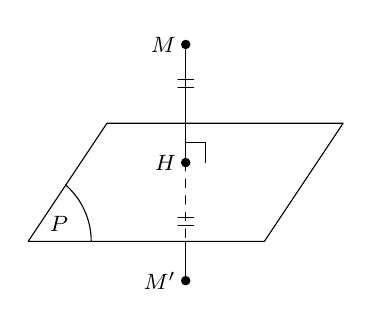
\begin{tikzpicture}[scale=0.5, font=\footnotesize,line join=round, line cap=round, >=stealth]
		\draw (0,0)--(-2,-3)--(4,-3)--(6,0)--cycle;
		\draw (2,2)--(2,-1) (2,-3)--(2,-4);
		\draw (2,-0.5)--(2.5,-0.5)--(2.5,-1);
		\draw (1.8,1.1)--(2.2,1.1) (1.8,0.9)--(2.2,0.9);
		\draw (1.8,-2.4)--(2.2,-2.4) (1.8,-2.6)--(2.2,-2.6);
		\draw[dashed] (2,-1)--(2,-3);
		\draw (-2+0.3,-3) node[above right] {$P$};
		\draw[fill=black] (2,-4) circle(3pt) node[left] {$M'$};
		\draw[fill=black] (2,2) circle(3pt) node[left] {$M$};
		\draw[fill=black] (2,-1) circle(3pt) node[left] {$H$};
		\draw (-0.4,-3) arc(0:49:1.9);
	\end{tikzpicture}
\end{center}
\textbf{Lưu ý: } Để tìm điểm đối xứng $M'$ của điểm $M$ qua $(P) \Rightarrow H$ là trung điểm của $MM'$.
\textbf{2. Tìm hình chiếu $H$ của điểm $M$ lên đường thẳng $d$}
Viết phương trình mặt phẳng $(P)$ qua $M$ và vuông góc với $d$, khi đó
$H = d \cap (P)$ thỏa $\heva{&x=x_0+a_1t\\&y=y_0+a_2t\\&z=z_0+a_3t\\&ax+by+cz+d=0\\} \Rightarrow \heva{&x=?\\&y=?\\&z=?\\} \Rightarrow H$.
\begin{center}
	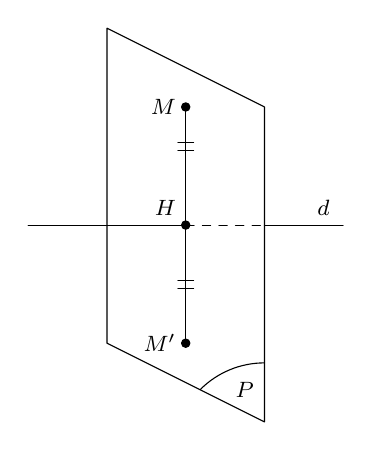
\begin{tikzpicture}[scale=0.5, font=\footnotesize,line join=round, line cap=round, >=stealth]
		\draw (0,4)--(0,-4)--(4,-6)--(4,2)--cycle;
		\draw (2,2)--(2,-4);
		\draw (1.8,1.1)--(2.2,1.1) (1.8,0.9)--(2.2,0.9);
		\draw (1.8,-2.4)--(2.2,-2.4) (1.8,-2.6)--(2.2,-2.6);
		\draw (-2,-1)--(2,-1) (4,-1)--(6,-1);
		\draw[dashed] (2,-1)--(4,-1);
		\draw (4-0.5,-6+0.8) node {$P$};
		\draw (4,-4.5) arc(90:135:2.3);
		\draw[fill=black] (2,-4) circle(3pt) node[left] {$M'$};
		\draw[fill=black] (2,2) circle(3pt) node[left] {$M$};
		\draw[fill=black] (2,-1) circle(3pt) node[above left] {$H$};
		\draw[fill=black] (5.5,-1) node[above] {$d$};
	\end{tikzpicture}
\end{center}
\textbf{Lưu ý: } Để tìm điểm đối xứng $M'$ của điểm $M$ qua $d \Rightarrow H$ là trung điểm của $MM'$.
\end{dang}
%Cau-61
\begin{ex}%[2H5H2-6]
	Trong KG $Oxyz$, khoảng cách từ điểm $M\left(2; -4; -1\right)$ tới đường thẳng $\Delta \colon \heva{
		& x=t \\ 
		& y=2-t \\ 
		& z=3+2t \\ 
	}$ bằng
	\choice
	{$\sqrt{14}$}
	{$\sqrt{6}$}
	{\True $2\sqrt{14}$}
	{$2\sqrt{6}$}
	\loigiai{
		Đường thẳng $\Delta $ đi qua $N\left(0; 2; 3\right)$, có véc-tơ chỉ phương $\overrightarrow{u}=\left(1; -1; 2\right)$.\\
		$\overrightarrow{MN}=\left(-2;6;4\right);\ \left[\overrightarrow{MN},\overrightarrow{u}\right]=\left(16;8;-4\right)$.\\
		$\mathrm{d}\left(M,\Delta \right)=\dfrac{\left| \left[ \overrightarrow{MN},\overrightarrow{u} \right] \right|}{\left| \overrightarrow{u} \right|}=\dfrac{\sqrt{336}}{\sqrt{6}}=2\sqrt{14}.$
	}
\end{ex}
%Cau-62
\begin{ex}%[2H5V2-6]
	Trong KG $Oxyz$, tọa độ hình chiếu vuông góc của $M\left(1;0;1 \right)$ lên đường thẳng $\left( \Delta  \right) \colon \dfrac{x}{1}=\dfrac{y}{2}=\dfrac{z}{3}$ là
	\choice
	{$\left( 2;4;6 \right)$}
	{$\left( 1;\dfrac{1}{2};\dfrac{1}{3} \right)$}
	{$\left( 0;0;0 \right)$}
	{\True $\left( \dfrac{2}{7};\dfrac{4}{7};\dfrac{6}{7} \right)$}
	\loigiai{
		Đường thẳng $\Delta $ có véc-tơ chỉ phương $\overrightarrow{u}=\left( 1;2;3 \right)$ và có PTTS là $\heva{
			x=t  \\
			y=2t  \\
			z=3t  \\
		}\left( t\in \mathbb{R} \right)$.\\
		Gọi $N\left( t;2t;3t \right)\in \Delta $ là hình chiếu vuông góc của $M$ lên $\Delta $, khi đó\\
		$\overrightarrow{MN} \cdot \overrightarrow{u}=0\Leftrightarrow (t-1)+(2t-0)\cdot 2+(3t-1)\cdot 3=0\Leftrightarrow 14t-4=0\Leftrightarrow t=\dfrac{2}{7}\Rightarrow N\left( \dfrac{2}{7};\dfrac{4}{7};\dfrac{6}{7} \right)$.
	}
\end{ex}
%Cau-63
\begin{ex}%[2H5V2-6]
	Trong KG $Oxyz$, cho điểm $M(-4;0;0)$ và đường thẳng $\Delta \colon \heva{
		& x=1-t \\ 
		& y=-2+3t \\ 
		& z=-2t \\ 
	}$. Gọi $H(a;b;c)$ là hình chiếu của $M$ lên $\Delta $. Tính $a+b+c$.
	\choice
	{$5$}
	{\True $-1$}
	{$-3$}
	{$7$}
	\loigiai{
		Gọi $H$ là hình chiếu của $M$ lên $\Delta $ nên tọa độ của $H$ có dạng $H(1-t;-2+3t;-2t)$ và $\overrightarrow{MH}\perp \overrightarrow{u}_{\Delta}$.\\
		$\Rightarrow \overrightarrow{MH} \cdot \overrightarrow{u}_{\Delta }=0\Leftrightarrow 14t-11=0\Leftrightarrow t=\dfrac{11}{14}\Rightarrow H\left(\dfrac{3}{14};\dfrac{5}{14};\dfrac{-22}{14}\right)\Rightarrow a+b+c=-1$.
	}
\end{ex}
%Cau-64
\begin{ex}%[2H5V2-4]
	Trong KG $Oxyz$, tọa độ hình chiếu vuông góc của điểm $A\left( 3;2;-1 \right)$ lên mặt phẳng $\left( \alpha  \right)\colon x+y+z=0$ là
	\choice
	{$\left( -2;1;1 \right)$}
	{\True $\left( \dfrac{5}{3};\dfrac{2}{3};-\dfrac{7}{3} \right)$}
	{$\left( 1;1;-2 \right)$}
	{$\left( \dfrac{1}{2};\dfrac{1}{4};\dfrac{1}{4} \right)$}
	\loigiai{
		Gọi $H$ là hình chiếu của $A\left( 3;2;-1 \right)$ lên mặt phẳng $\left( \alpha  \right)\colon x+y+z=0$. Khi đó $AH$ nhận $\overrightarrow{n}=\left( 1;1;1 \right)$ là vectơ chỉ phương.\\
		Suy ra phương trình $AH \colon \dfrac{x-3}{1}=\dfrac{y-2}{1}=\dfrac{z+1}{1}$.\\
		Do $H\in AH\Rightarrow H\left( 3+t;2+t;-1+t \right)$.\\
		Do $H\in \left( \alpha  \right)\Rightarrow 3+t+2+t-1+t=0\Leftrightarrow t=-\dfrac{4}{3}\Rightarrow H\left( \dfrac{5}{3};\dfrac{2}{3};-\dfrac{7}{3} \right)$.
	}
\end{ex}
%Cau-65
\begin{ex}%[2H5V2-5]
	Trong không gian với hệ trục tọa độ $Oxyz$, hình chiếu của điểm $M\left( -1;0;3 \right)$ theo phương vectơ $\overrightarrow{v}=\left( 1;-2;1 \right)$ trên mặt phẳng $\left( P \right) \colon x-y+z+2=0$ có tọa độ là
	\choice
	{$\left( 2;-2;-2 \right)$}
	{$\left( -1;0;1 \right)$}
	{\True $\left( -2;2;2 \right)$}
	{$\left( 1;0;-1 \right)$}
	\loigiai{
		\begin{center}
			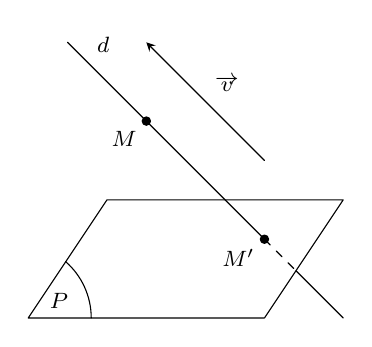
\begin{tikzpicture}[scale=0.5, font=\footnotesize,line join=round, line cap=round, >=stealth]
				\draw (0,0)--(-2,-3)--(4,-3)--(6,0)--cycle;
				\draw (-1,4)--(4,-1) (4.8,-1.8)--(6,-3);
				\draw[dashed] (4,-1)--(4.8,-1.8);
				\draw[->] (4,1)--(1,4);
				\draw (-2+0.3,-3) node[above right] {$P$};
				\draw[fill=black] (4,-1) circle(3pt) node[below left] {$M'$};
				\draw[fill=black] (1,2) circle(3pt) node[below left] {$M$};
				\draw (-0.5,3.5) node[above right] {$d$};
				\draw (2.5,2.5) node[above right] {$\overrightarrow{v}$};
				\draw (-0.4,-3) arc(0:49:1.9);
			\end{tikzpicture}
		\end{center}
		Đường thẳng $d$ đi qua $M\left( -1;0;3 \right)$, có véc-tơ chỉ phương $\overrightarrow{v}=\left( 1;-2;1 \right)$ có PTTS là $\heva{
			& x=-1+t \\ 
			& y=-2t \\ 
			& z=3+t. \\ 
		}$\\
		Gọi $M'$ là hình chiếu của điểm $M\left( -1;0;3 \right)$ theo phương véc-tơ $\overrightarrow{v}=\left( 1;-2;1 \right)$ trên mặt phẳng $\left( P \right) \colon x-y+z+2=0$.\\
		$\Rightarrow M'=d\cap \left( P \right)\Rightarrow $ tọa độ $M'$ là nghiệm của hệ phương trình\\
		$\heva{
			& x=-1+t \\ 
			& y=-2t \\ 
			& z=3+t \\ 
			& x-y+z+2=0 \\ 
		}\Leftrightarrow \heva{
			& x=-1+t \\ 
			& y=-2t \\ 
			& z=3+t \\ 
			& -1+t+2t+3+t+2=0 \\ 
		}\Leftrightarrow \heva{
			& x=-2 \\ 
			& y=2 \\ 
			& z=2 \\ 
			& t=-1 \\ 
		}\Rightarrow M'\left( -2;2;2 \right)$.
		
	}
\end{ex}
%Cau-66
\begin{ex}%[2H5V2-5]
	Trong KG $Oxyz$, cho mặt phẳng $\left( P \right) \colon 6x-2y+z-35=0$ và điểm $A\left( -1;3;6 \right).$ Gọi $A'$ là điểm đối xứng với $A$ qua $\left( P \right)$, tính $OA'.$
	\choice
	{$OA'=5\sqrt{3}$}
	{$OA'=\sqrt{46}$}
	{\True $OA'=\sqrt{186}$}
	{$OA'=3\sqrt{26}$}
	\loigiai{
		$A'$ đối xứng với $A$ qua $\left( P \right)$ nên $AA'$ vuông góc với $\left( P \right)$.\\
		Suy ra PTĐT $AA' \colon \heva{
			& x=-1+6t \\ 
			& y=3-2t \\ 
			& z=6+t. \\ 
		}$\\
		Gọi $H$ là giao điểm của $AA'$ và mặt phẳng $\left( P \right) \Rightarrow H\left( -1+6t;3-2t;6+t \right)$.\\
		Do $H$ thuộc $\left( P \right) \Rightarrow 6\left( -1+6t \right)-2\left( 3-2t \right)+1\left( 6+t \right)-35=0 $.\\
		$\Leftrightarrow 41t-41=0\Leftrightarrow t=1\Rightarrow H\left( 5;1;7 \right)$.\\
		$A'$ đối xứng với $A$ qua $\left( P \right)$ nên $H$ là trung điểm của $AA'\Rightarrow {A}'\left( 11;-1;8 \right)\Rightarrow OA'=\sqrt{11^2+\left( -1 \right)^2+8^2}=\sqrt{186}$.
	}
\end{ex}
%Cau-67
\begin{ex}%[2H5V2-2]
	Trong KG $Oxyz$, cho đường thẳng $d \colon \dfrac{x-1}{1} = \dfrac{y-1}{2} = \dfrac{z-2}{-1}$ và mặt phẳng $(P) \colon 2x+y+2z-1=0$. Gọi $d'$ là hình chiếu của đường thẳng $d$ lên mặt phẳng $(P)$, véc-tơ  chỉ phương của đường thẳng $d'$ là
	\choice
	{$\overrightarrow{u}_3 = (5;-6;-13)$}
	{$\overrightarrow{u}_2 = (5;-4;-3)$}
	{$\overrightarrow{u}_4 = (5;16;13)$}
	{\True $\overrightarrow{u}_1 = (5;16;-13)$}
	\loigiai{
		Đường thẳng $d$ đi qua điểm $A(1;1;2)$ và có một véc-tơ chỉ phương $\overrightarrow{u}_d = (1;2;-1)$.\\
		Mặt phẳng $(P)$ có một véc-tơ pháp tuyến $\overrightarrow{n}_{(P)}= (2;1;2)$.\\
		Gọi $\overrightarrow{u}_{d'}$ là một  véc-tơ chỉ phương của đường thẳng $d'$.\\
		Gọi $(Q)$ là mặt phẳng chứa đường thẳng $d$ và vuông góc với mặt phẳng $(P)$. Khi đó, $(Q)$ đi qua điểm $A(1;1;2)$ và có một véc-tơ pháp tuyến $\overrightarrow{n}_{(Q)} = \left[\overrightarrow{u}_d, \overrightarrow{u}_{(P)}\right] = (5;-4;-3)$.\\
		Đường thẳng $d'$ là hình chiếu của đường thẳng $d$ trên mặt phẳng $(P) \Leftrightarrow d' = (P) \cap (Q)$ nên  $\heva{&\overrightarrow{u}_{d'} \perp \overrightarrow{n}_{(P)}\\&\overrightarrow{u}_{d'} \perp \overrightarrow{n}_{(Q)}.}$\\
		Véc-tơ chỉ phương của đường thẳng $d'$ là $\overrightarrow{u}_{d'}=\left[\overrightarrow{n}_{(P)}, \overrightarrow{n}_{(Q)}\right] =(5;16;-13)$.
	}
\end{ex}
%Cau-68
\begin{ex}%[2H5V2-3]
	Trong KG $Oxyz$, cho mặt phẳng $(\alpha) \colon 2x+y+z-3=0$ và đường thẳng $d\colon \dfrac{x+4}{3} = \dfrac{y-3}{-6} = \dfrac{z-2}{-1}$. Viết PTĐT $d'$ đối xứng với đường thẳng $d$ qua mặt phẳng $(\alpha)$.
	\choice
	{$\dfrac{x}{11} = \dfrac{y+5}{-17} = \dfrac{z-4}{-2}$}
	{$\dfrac{x}{11} = \dfrac{y-5}{-17} = \dfrac{z+4}{-2}$}
	{\True $\dfrac{x}{11} = \dfrac{y-5}{-17} = \dfrac{z-4}{-2}$}
	{$\dfrac{x}{11} = \dfrac{y-5}{-17} = \dfrac{z-4}{2}$}
	\loigiai{
		Mặt phẳng $(\alpha) \colon 2x+y+z-3=0$ có véc-tơ pháp tuyến là $\overrightarrow{n} = (2;1;1)$.\\
		Gọi tọa độ giao điểm của $d$ và $(\alpha)$ là $I$ thì $I(-22;39;8)$.\\
		Lấy $A(-4;3;2) \in d$. Gọi $\Delta$ là đường thẳng đi qua $A$ và vuông góc với $(\alpha)$.\\
		Suy ra PTĐT $\Delta \colon \heva{&x=-4+2t\\&y=3+t\\&z=2+t.\\}$\\
		Gọi $H$ là hình chiếu của $A$ lên $(\alpha)$ thì $H = \Delta \cap (\alpha)\Rightarrow H(-2;4;3)$.\\
		$A'$ đối xứng với $A$ qua $(\alpha) \Leftrightarrow H$ là trung điểm của $AA'$, $d'$ có véc-tơ chỉ phương $\overrightarrow{A'I} = (22;-34;-4) = 2(11;-17;-2)$ có phương trình là $\dfrac{x}{11} = \dfrac{y-5}{-17} = \dfrac{z-4}{-2}$.
	}
\end{ex}
%Cau-69
\begin{ex}%[2H5C2-3]
	Trong KG $Oxyz$, cho đường thẳng $d \colon \dfrac{x-1}{2} = \dfrac{y+5}{-1} = \dfrac{z-3}{4}$. Phương trình nào dưới đây là phương trình hình chiếu vuông góc của $d$ trên mặt phẳng $x+3=0$?
	\choice
	{$\heva{&x=-3\\&y=-5+2t\\&z=3-t\\}$}
	{\True $\heva{&x=-3\\&y=-6-t\\&z=7+4t\\}$}
	{$\heva{&x=-3\\&y=-5-t\\&z=-3+4t\\}$}
	{$\heva{&x=-3\\&y=-5+t\\&z=3+4t\\}$}
	\loigiai{
		Đường thẳng $d$ đi qua điểm $M_0(1;-5;3)$ và có véc-tơ chỉ phương $\overrightarrow{u}_d=(2;-1;4)$.\\
		Gọi $(Q)$ là mặt phẳng chứa $d$ và vuông góc với $(P) \colon x + 3 = 0$.\\
		Suy ra mặt phẳng $(Q)$ đi qua điểm $M_0(1;-5;3)$ và có véc-tơ pháp tuyến là $\left[\overrightarrow{n}_{(P)}; \overrightarrow{u}_d\right] = (0;4;1)$.\\
		$\Rightarrow (Q) \colon 4y+z+17=0$.\\
		Phương trình hình chiếu của $d$ lên mặt phẳng $(P)$ là \\
		$$\heva{&4y+z+17=0\\&x+3=0} \text{hay} \heva{&x=-3\\&y=-6-t\\&z=7+4t.}$$\\
 	}
\end{ex}
%Cau-70
\begin{ex}%[2H5C2-3]
	Trong KG $Oxyz$, cho mặt phẳng $(P) \colon x+y+z-3=0$ và đường thẳng $d \colon \dfrac{x}{1} = \dfrac{y+1}{2} = \dfrac{z-2}{-1}$. Hình chiếu vuông góc của $d$ trên $(P)$ có phương trình là
	\choice
	{\True $\dfrac{x-1}{1} = \dfrac{y-1}{4} = \dfrac{z-1}{-5}$}
	{$\dfrac{x-1}{1} = \dfrac{y-1}{4} = \dfrac{z+5}{1}$}
	{$\dfrac{x+1}{-1} = \dfrac{y+1}{-4} = \dfrac{z+1}{5}$}
	{$\dfrac{x-1}{3} = \dfrac{y-1}{-2} = \dfrac{z-1}{-1}$}
	\loigiai{
		Gọi $M$ là giao điểm của $d$ và $(P)$.\\
		Tọa độ của $M$ là nghiệm của hệ $$\heva{&x+y+z-3=0\\&\dfrac{x}{1} = \dfrac{y+1}{2} = \dfrac{z-2}{-1}\\} \Leftrightarrow \heva{&x+y+z=3\\&2x-y=1\\&x+z=2\\}\Leftrightarrow \heva{&x=1\\&y=1\\&z=1\\} \Rightarrow M(1;1;1).$$
		Lấy điểm $N(0;-1;2) \in d$.\\
		Một véc-tơ pháp tuyến của mặt phẳng $(P)$ là $\overrightarrow{n} = (1;1;1)$.\\
		Gọi $\Delta$ là đường thẳng đi qua $N$ và nhận $\overrightarrow{n}=(1;1;1)$ làm véc-tơ chỉ phương.\\
		PTĐT $\Delta \colon \dfrac{x}{1} = \dfrac{y+1}{1} = \dfrac{z-2}{1}$.\\
		Gọi $N'$ là giao điểm của $\Delta$ với $(P)$.\\
		Tọa độ của $N'$ là nghiệm của hệ
		$$\heva{&x+y+z-3=0\\&\dfrac{x}{1} = \dfrac{y+1}{1} = \dfrac{z-2}{1}\\} \Leftrightarrow \heva{&x+y+z=3\\&x-y=1\\&x-z=-2\\} \Leftrightarrow \heva{&x=\dfrac{2}{3}\\&y=-\dfrac{1}{3}\\&z=\dfrac{8}{3}} \Rightarrow N'\left(\dfrac{2}{3};-\dfrac{1}{8};\dfrac{8}{3}\right).$$
		$\overrightarrow{MN'} = \left(-\dfrac{1}{3};-\dfrac{4}{3};\dfrac{5}{3}\right) = -\dfrac{1}{3}(1;4;-5)$.\\
		Đường thẳng cần tìm đi qua điểm $M(1;1;1)$ và nhận $\overrightarrow{u} = (1;4;-5)$ làm véc-tơ chỉ phương nên có phương trình $\dfrac{x-1}{1} = \dfrac{y-1}{4} = \dfrac{z-1}{-5}$.
	}
\end{ex}
%Cau-71
\begin{ex}%[2H5C2-3]
	Trong KG $Oxyz$, cho mặt phẳng $(P) \colon x+y-z-1=0$ và đường thẳng $d \colon \dfrac{x+2}{2} = \dfrac{y-4}{-2} = \dfrac{z+1}{1}$. Viết PTĐT $d'$ là hình chiếu vuông góc của $d$ lên $(P)$.
	\choice
	{$d' \colon \dfrac{x+2}{7} = \dfrac{y}{-5} = \dfrac{z+1}{2}$}
	{\True $d' \colon \dfrac{x-2}{7} = \dfrac{y}{-5} = \dfrac{z-1}{2}$}
	{$d' \colon \dfrac{x+2}{7} = \dfrac{y}{5} = \dfrac{z+1}{2}$}
	{$d' \colon \dfrac{x-2}{7} = \dfrac{y}{5} = \dfrac{z-1}{2}$}
	\loigiai{
		PTTS của $d \colon \heva{&x=-2+2t\\&y=4-2t\\&z=-1+t\\}, \ t \in \mathbb{R}$. \\
		Gọi $M = (-2+2t;4-2t;-1+t)$  là giao điểm của $d$ và $(P)$.\\
		$\Rightarrow (-2+2t) + (4-2t) - (-1+t) - 1 = 0 \Leftrightarrow t = 2 \Rightarrow M=( 2;0;1)$.\\
		Mặt phẳng $(P)$ có một véc-tơ pháp tuyến là $\overrightarrow{n}_{(P)} = (1;1;-1)$. Điểm $N = (0;2;0) \in d$.\\
		Gọi $\Delta$ là đường thẳng đi qua $N(0;2;0)$ và vuông góc với mặt phẳng $(P) \Rightarrow \Delta$ nhận $\overrightarrow{n}_{(P)} = (1;1;-1)$ làm véc-tơ chỉ phương. Suy ra phương trình của $\Delta$ là
		$$\Delta \colon \dfrac{x-0}{1} = \dfrac{y-2}{1} = \dfrac{z-0}{-1} \Leftrightarrow \Delta \colon \heva{&x=c\\&y=2+c\\&z=-c\\}, \ c \in \mathbb{R}.$$
		Gọi $M'=(c;2+c;-c)$ là giao điểm của $\Delta$  với mặt phẳng $(P) \Rightarrow c+(2+c)-(-c)-1=0 \Leftrightarrow c=-\dfrac{1}{3} \Rightarrow M'\left(-\dfrac{1}{3};\dfrac{5}{3};\dfrac{1}{3}\right)$.\\
		$\overrightarrow{MM'}=\left(-\dfrac{7}{3};\dfrac{5}{3};-\dfrac{2}{3}\right)$, đường thẳng $d'$ là hình chiếu vuông góc của $d$ trên mặt phẳng $(P)$ nên $d'$ chính là đường thẳng $MM'$, suy ra $d'$ đi qua $M(2;0;1)$ và nhận véc-tơ $\overrightarrow{u} = -3\overrightarrow{MM'}=(7;-5;2)$ làm véc-tơ chỉ phương nên phương trình của $d'$ là\\
		$d' \colon \dfrac{x-2}{7} = \dfrac{y}{-5} = \dfrac{z-1}{2}$.
	}
\end{ex}
\Closesolutionfile{ans}
\indapan{10}{ans/ans-2-C5B3CD3-32-41}